\documentclass[10pt]{article}
\usepackage{float}
\usepackage{amsmath}
\usepackage{paralist}
\usepackage{setspace}
\usepackage{listings}
\usepackage{graphicx}
\usepackage[english]{babel}
\usepackage{geometry}
\usepackage{subcaption}
\usepackage[utf8]{inputenc}
\usepackage{listings}
\usepackage{color}
\usepackage{subcaption}
\usepackage{hyperref}
\usepackage{eurosym}



\begin{document}


\definecolor{mygreen}{rgb}{0,0.6,0}
\definecolor{mygray}{rgb}{0.5,0.5,0.5}
\definecolor{mymauve}{rgb}{0.58,0,0.82}

\lstset{ %
  backgroundcolor=\color{white},   % choose the background color; you must add \usepackage{color} or \usepackage{xcolor}
  basicstyle=\footnotesize,        % the size of the fonts that are used for the code
  breakatwhitespace=false,         % sets if automatic breaks should only happen at whitespace
  breaklines=true,                 % sets automatic line breaking
  captionpos=b,                    % sets the caption-position to bottom
  commentstyle=\color{mygreen},    % comment style
  deletekeywords={...},            % if you want to delete keywords from the given language
  escapeinside={\%*}{*)},          % if you want to add LaTeX within your code
  extendedchars=true,              % lets you use non-ASCII characters; for 8-bits encodings only, does not work with UTF-8
  frame=tb,	                   % adds a frame around the code
  keepspaces=true,                 % keeps spaces in text, useful for keeping indentation of code (possibly needs columns=flexible)
  keywordstyle=\color{blue},       % keyword style
  language=Octave,                 % the language of the code
  otherkeywords={*,...},           % if you want to add more keywords to the set
  numbers=left,                    % where to put the line-numbers; possible values are (none, left, right)
  numbersep=5pt,                   % how far the line-numbers are from the code
  numberstyle=\tiny\color{mygray}, % the style that is used for the line-numbers
  rulecolor=\color{black},         % if not set, the frame-color may be changed on line-breaks within not-black text (e.g. comments (green here))
  showspaces=false,                % show spaces everywhere adding particular underscores; it overrides 'showstringspaces'
  showstringspaces=false,          % underline spaces within strings only
  showtabs=false,                  % show tabs within strings adding particular underscores
  stepnumber=2,                    % the step between two line-numbers. If it's 1, each line will be numbered
  stringstyle=\color{mymauve},     % string literal style
  tabsize=2,	                   % sets default tabsize to 2 spaces
  title=\lstname                   % show the filename of files included with \lstinputlisting; also try caption instead of title
}

\onehalfspacing


\section{CIP 4}

The following parameters are relevant for the remainder of this section:

\begin{align*}
	\Omega_{rated} &= 12.59 rpm \text{ (rotor rated speed)} \\
	D &= 5m \text{ (tower diameter)} \\
	E &=211000000000 \frac{N}{m^2} \text{ (elastic modulus)} \\
	l &=100m \text{ (hub height)} \\
	m_{top} &=323000 kg\text{ (nacelle and rotor mass)} \\
	\rho &=7850 \frac{kg}{m^3}\text{ (material density)} \\
\end{align*}

\subsection{Task a}
For tower design resonances of excitation frequencies from the rotating blades must be taken into account. The Eigenfrequency of the tower can thus be obtained by adding a $10 \%$ safety margin to the rotor rated speed which represents the maximum stationary rotor speed:
\begin{equation*}
	f_0 = \Omega_{rated} \cdot 1.1 = \frac{12.59}{60} Hz \cdot 1.1 = 0.23081 Hz
\end{equation*}

\subsection{Task b}
The design range of our turbine is a classical soft-stiff design which results in large wave excitation.

\subsection{Task c}
The wall thickness $t$ can be computed from the following equations:

\begin{align}
f_0 \ccot 2 \pi &= \sqrt{\frac{k}{m_{top} + 0.25 m_{tower}}} \\
k &= \frac{3 E \pi D^3 t}{l^3 8} \\
m_{tower} &= \rho \pi D t l
\end{align}

By substituting Equations (2) and (3) into (1) we obtain the following equality which can be fed into Matlab in order to solve for the only unknown $t$:\\

\begin{equation*}
0 = \sqrt{\frac{3 E \pi D^3 t}{l^3 8 \cdot (m_{top} + 0.25\rho \pi D t l)}} -f_0 \cdot 2 \pi \\
\end{equation*}

Extract from Matlab code used to solve for variable $t$:\\

\begin{lstlisting}
t=1;
func = @(t) sqrt(3*E*pi*D^3*t/(l^3*8*(mTop+0.25*rho*pi*D+t*l)))-0.23081*2*pi;
t = fsolve(func,t);
\end{lstlisting}

The resulting value for the wall thickness is $t=0.0239m$. The tower mass is then $m_{tower}=295310 kg = 295.31t$. The material cost for this tower would thus be of $147655$ \euro, assuming a price of $500$ \euro /t. Obviously a thicker tower wall leads to a higher price overall (linear increase). As depicted in Figure~\ref{fig:eigfreqWall} a thicker wall leads to a higher Eigenfrequency of the tower as well. However, in this case the relationship is not a linear one due to the exponent of $0.5$ in the formula. Hence, a thicker wall results in a higher Eigenfrequency but the increase is only significant for wall thicknesses up to $0.1m$. Above that the cost increase does not justify the gain in Eigenfrequency.

\begin{figure}[H]
\centering
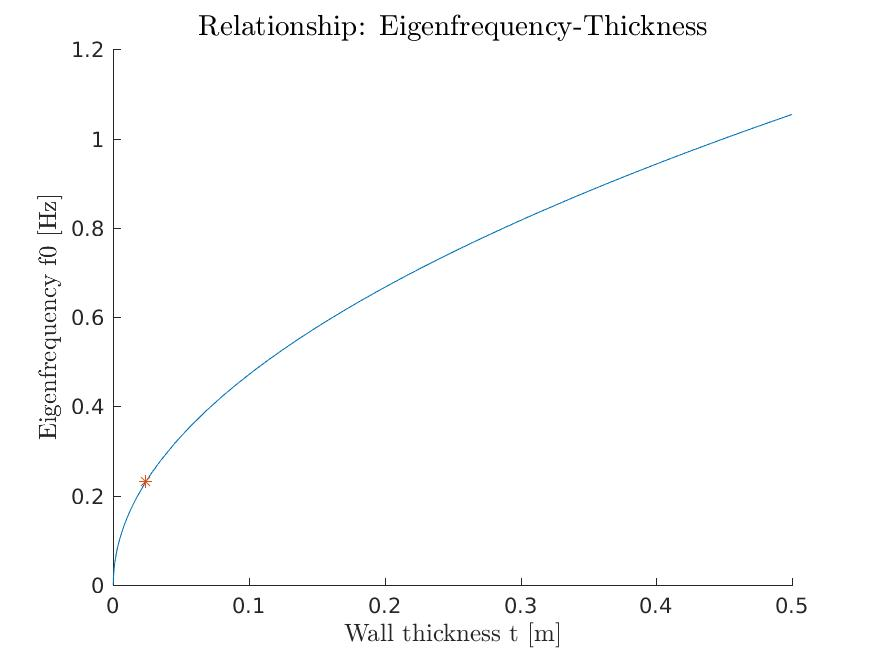
\includegraphics[width=0.6\linewidth]{../figures/eigenfrequency.jpg}
\caption{Effect of wall thickness on Eigenfrequencies}
\label{fig:eigfreqWall}
\end{figure} 

\subsection{Task d}
The Campbell diagram is depicted in Figure~\ref{fig:campbell}  (work in progress)
\begin{figure}[H]
\centering
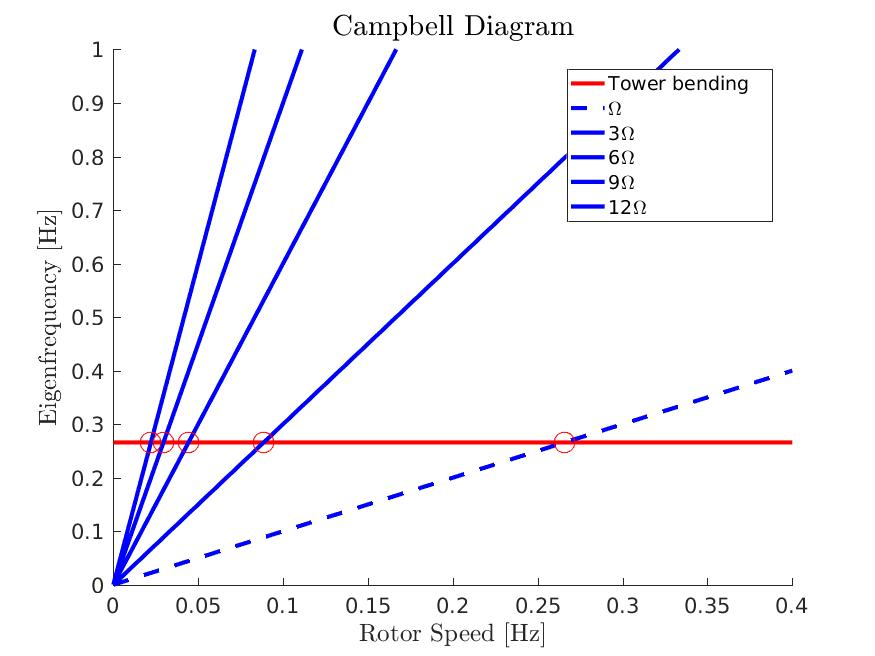
\includegraphics[width=1\linewidth]{../figures/campbell.jpg}
\caption{Campbell Diagram}
\label{fig:campbell}
\end{figure} 
\end{document}